%\documentclass[ngerman,dvips]{wkcms}  % latex + dvips
\documentclass[ngerman,pdf]{wkcms}    % pdflatex

\usepackage[utf8]{inputenc}

\title{SSH - The Secure Shell}
\subtitle{Überblick, Technologie, Anwendungsbeispiele}
\author{Susanne Kießling}
\date{\todaylong}

\address
{Hochschule Augsburg\\
 Masterstudiengang Informatik\\
 E-Mail: \url{susanne.kiessling@hs-augsburg.de}      
}

\begin{abstract}
Test, Test, Test ...
Dfsjkhc sdjfh sdjlkfh sdljkf hlasdjkf haljksdfh asdjlfh als. asdfjk asdjflkha
sdfljhas dfljashd fljkasdhf jlaksdfh lajskdfh alsjkdfh asldjkf hasldjkfh
asljkdfh asljkdf hasljdkfh asljkdfh asljkdfh asljkdfh asljkdfh asljkdfh
asljkdfh alsjkdfh asljkdfh asljkdfh asljkdfh asljkdfh asldkjfh asldkjfh
aslkdjfh.

Asljkdfh alsjkdfh asljkdfh asljkdfh asljkdfh asljkdfh asldkjfh asldkjfh
asljkdfh alsjkdfh asljkdfh asljkdfh asljkdfh asljkdfh asldkjfh asldkjfh
asljkdfh alsjkdfh asljkdfh asljkdfh asljkdfh asljkdfh asldkjfh asldkjfh
aslkdjfh.
\end{abstract}

\keywords{Content Management, Database}
\categories{Allgemein}

\begin{document}

\maketitle


\section{Einleitung}

Die Übertragung von Daten innerhalb von Computernetzwerken geschieht ohne
entsprechende Vorkehrungen grundsätzlich ungesichert. E-Mails, Passwörter und sämtliche Daten, die übertragen werden, können abgefangen und gelesen werden. SSH (Secure Shell) ist ein Protokoll, das die verschlüsselte Übertragung von Daten über ein Netzwerk ermöglicht \cite{SSH}.
Trotz zahlreicher Berichterstattung über die Folgen von sorglosem Umgang mit Daten in Computernetzwerken, wozu natürlich auch das World Wide Web gehört, ändern viele Nutzer
ihr Verhalten diesbezüglich nicht. Die Sicherheit von privaten Daten ist ein hochaktuelles Thema. SSH (als Protokoll) und dessen Implementierungen stellen eine Möglichkeit dar, Daten innerhalb eines Computernetzwerks sicher zu übertragen. Ziel ist es nun, einen Überblick zu SSH zu geben. OpenSSH dient anschließend als Beispiel-Implementierung, anhand derer die Funktionalitäten gezeigt werden. Der Ablauf eines Verbindungsaufbaus und die verwendeten Verschlüsselungsalgorithmen werden gezeigt. Auf aktuelle sicherheitskritische BUGs wird eingegangen.

--> evtl. als aktuell erwähnen, dass es auch SSH für mobile Betriebssysteme gibt
--> 

 schlechte Passwörter/Bruce Schneier?
 

SSH (Secure Shell) ist eine unixoide \cite{knuthwebsite} Tralalala...


asljkdfh asljkdfh alskjdfh lajskdfh. dasdkf hjasdfh adköshf asjlkdf
hasjldkf hlasjkdfh jl hasdljka shdfasdfa sdfasdf\footnote{sdfsdfs dsfsdfsd}



\newpage

\section{Grundprinzip von SSH}
\bzgl \bzw \ca \Dh \evtl \etc \ggf \iAllg \oAe \uAe \usf \usw \vgl \zB \\
\cf \cp \ie \eg \etc \wrt \viz \vs \Wlog \\
\PF{"a"} \\
\RM{bla} \TT{bla} \\
\BF{bla \MD{bla} bla} \\
\IT{bla \MD{bla} bla} \\
\SC{bla} \EM{bla} \\
\CAL{R} \\
\NT{ein Terminal} $\Blank \nin \{\}$

SSH verschlüsselt die forlaufende Verbindung zwischen Computern in einem Netzwerk. Dazu verwendet SSH eine Client/Server-Architektur. 

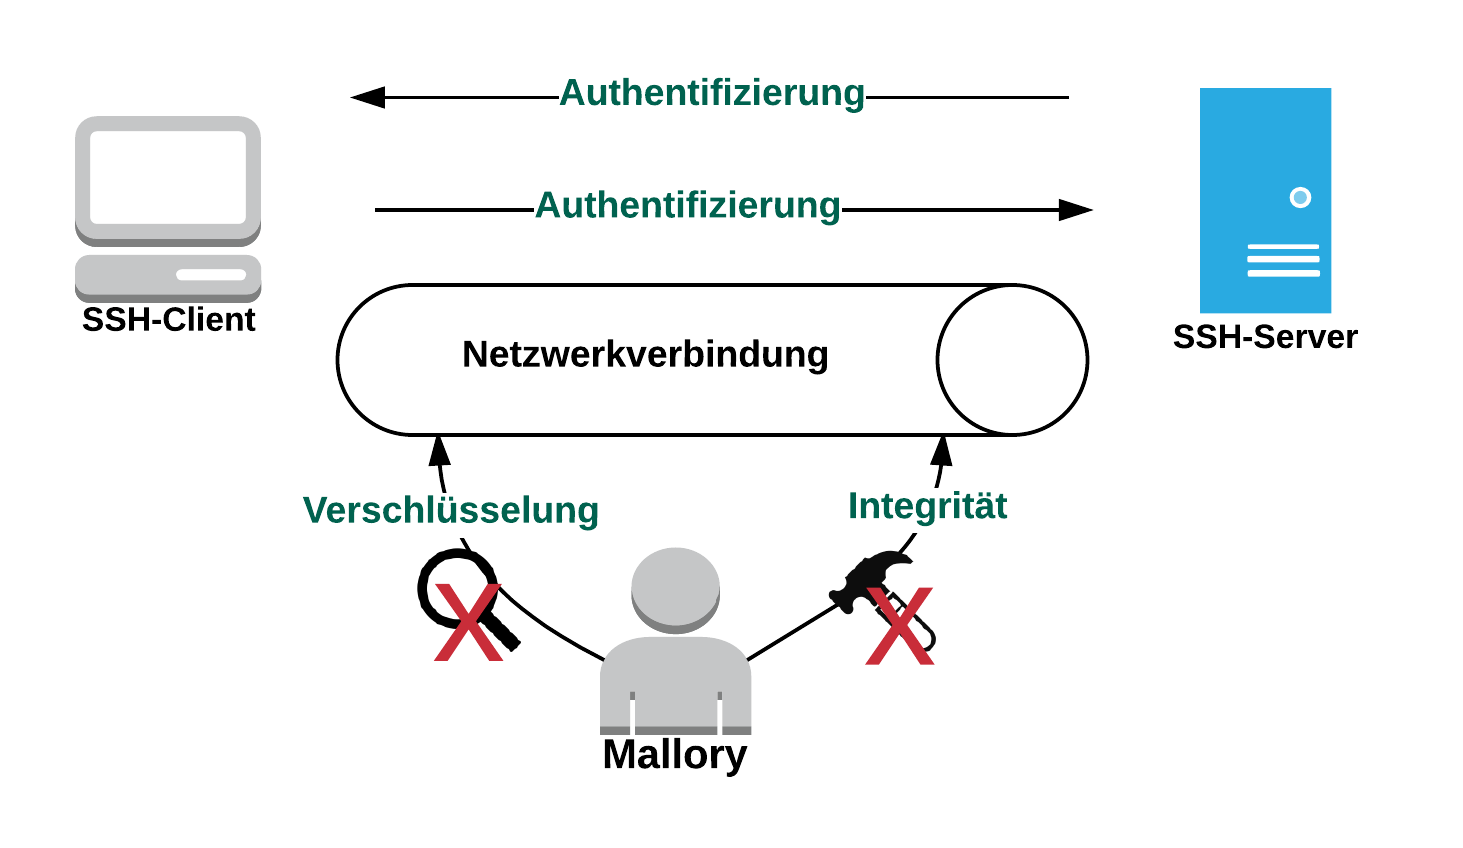
\includegraphics[width=\linewidth]{./images/grundprinzip.png}


\subsection{Protokolle}
SSH-1, SSH-2

\subsection{Implementierungen}

\paragraph{Dropbear} Ist eine Implementierung des SSH2-Protokolls und steht unter der MIT-Lizenz.
\paragraph{Mosh} Bietet weitere Funktionalitäten, vorallem für mobile Nutzer. Die Verbindung wird bei Roaming aufrecht erhalten. Zusätzlich bietet Mosh eine optimierte Latenz, \Dh ...
\paragraph{Lsh}
\paragraph{PuTTY} MIT-Lizenz, überwiegend für Windows.
\paragraph{OpenSSH}

\section{OpenSSH}

OpenSSH -- eine der bekanntesten Implemetierungen des SSH-Protokolls -- dient nun dazu,
elemnentare Funktionalitäten vorzustellen. 

--> beinhaltet Server und Client
--> einfaches Installieren über den Paketmanager

\subsection{Remote Terminal Session}

\begin{program}
[sue@kaktus]\$ ssh micra@login.rz.hs-augsburg.de
micra@login.rz.hs-augsburg.de's password:
%Linux bug 3.2.0-4-amd64 #1 SMP Debian 3.2.65-1+deb7u1 x86_64
Plan your installation, and FAI installs your plan.

Last login: Mon Apr 25 22:38:45 2016
from p5088ff5b.dip0.t-ipconnect.de
micra@bug:~\$

\end{program}

\subsection{Datenübertragung mit \IT{scp}}

\begin{program}
[sue@kaktus ~]\$ scp hello\_all.txt
micra@login.rz.hs-augsburg.de:~
micra@login.rz.hs-augsburg.de's password:
hello\_all.txt        100\% 6297     6.2KB/s   00:00
\end{program}

\subsection{Dateisystem einhängen mit \IT{sshfs}}

\begin{program}
sshfs [user@]host:[dir] mountpoint [options]
\end{program}

\subsection{Public-Key-Authentifizierung}
\subsection{Port-Forwarding}
\subsection{X-Forwarding}
\subsection{Agenten?}


\section{Sicherheitsrelevante Betrachtung}
\subsection{Verschlüsselungsalgorithmen bei SSH}
\subsection{Ablauf einer sicheren Verbindung}
\subsection{Aktuelle Schwachstellen}
\subsection{Anforderungen an den Serveradministrator}


\newpage


\section{Zusammenfassung}


\bibliography{sample}
\bibliographystyle{unsrt}


\end{document}


